\documentclass[conference]{IEEEtran}
\IEEEoverridecommandlockouts

\usepackage{cite}
\usepackage{graphicx}
\usepackage{booktabs}
\usepackage{array}
\usepackage{url}
\usepackage[T1]{fontenc}
\usepackage{textcomp}
\usepackage{upquote}
\newcommand{\code}[1]{\texttt{#1}}

\begin{document}

\title{Byte-Preserving Response Splitting to Obfuscate the Segmentation
Fingerprint of DNP3 Outstations}

\author{\IEEEauthorblockN{Author Name(s)}
\IEEEauthorblockA{Affiliation \\ Email address}}

\maketitle

\begin{abstract}
A passive observer of DNP3 traffic can tell one outstation from another without
ever reading a measurement value. What gives a device away is the shape of its
replies: how long a response runs, how it breaks into frames, and the spacing
between those frames. That shape holds steady, because a DNP3 outstation
assembles its frames the same way on every read, and it resists tampering. DNP3
guards each 16-byte block of a message with a CRC that the master rechecks while
reassembling, so editing the response bytes, padding them, or rewriting a length
field tends to trip a CRC and get the reply thrown out. We take a narrower route
that leaves every byte alone. The primitive, which we call CRC-boundary
splitting, re-cuts a captured response into TCP chunks only where a CRC block
already ends. No DNP3 field is altered and no CRC is recomputed; the chunks join
back into the exact original, and the live master rebuilds the same application
message it would have received from the device itself. We wrap the primitive in a
request-aware server that sits in the outstation's place, answers each request
with its own captured response, and splits every data response along its CRC
boundaries. On a two-host testbed running OpenDNP3, a large Class~0 read that the
outstation normally emits as 9~application fragments (49~link frames, 20~TCP
segments) instead left the wire as 141~chunks of no more than 18~bytes, and the
master still took every measurement and returned a DNP3 CONFIRM over a connection
with no retransmission and no reset. This held across the full range of splitting
we tried. We read that as reason to believe CRC-boundary splitting can serve as
the transparent building block for an in-network layer that blunts passive
fingerprinting of DNP3 outstations.
\end{abstract}

\begin{IEEEkeywords}
DNP3, SCADA, traffic obfuscation, device fingerprinting, industrial control
systems.
\end{IEEEkeywords}

\section{Introduction}

The grid runs on old protocols. Power utilities move their measurements and
control commands over protocols such as DNP3 (Distributed Network
Protocol~3)~\cite{ref:dnp3}, and DNP3, like most of its peers, ships with no
encryption and no authentication by default~\cite{ref:dnp3}. Anyone on the path
can therefore read the exchange. The cost of that exposure is not hypothetical.
In December~2015 a set of remote intruders reached into a Ukrainian power grid
and left 225{,}000 residents in the dark~\cite{ref:ukraine}. An attack of that
scale does not begin with the attack; it begins with watching, with learning
which devices are on the wire and how each one behaves. So what a quiet observer
can pull out of unencrypted control traffic is worth taking seriously, and not
only on paper.

Reading the payload is not even necessary. Traffic-analysis work has shown that
packet sizes and timing on their own are enough to recover the content of
encrypted sessions~\cite{ref:fp}, and unencrypted DNP3 hands over the same side
channel more cheaply. The length of a response, the count of frames it splits
into, and the gaps between those frames together make a fingerprint of the device
and of its point database. A large integrity poll, for instance, comes back long
and heavily segmented, while a small point read comes back short, so the
segmentation an observer sees already discloses roughly how many points the
device carries. Because the outstation lays out its frames deterministically,
that fingerprint tends to stay put from one session to the next. An observer can
then sort device types apart, guess database sizes, and follow a device across
sessions, and none of it requires breaking a cipher.

Erasing the fingerprint is hard, for two reasons. First, DNP3 wraps every 16-byte
block of an application message in a CRC, and the master checks those CRCs as it
reassembles, so any edit to the response bytes, any padding slipped in, or any
length field rewritten runs the risk of a CRC failure that the master simply
rejects. Second, the outstation firmware is fixed and comes from the vendor, so
nothing a practical defense does can change how the device itself frames its
data. That leaves a gap: we lack a primitive that reshapes the size and
segmentation a DNP3 response shows on the wire yet still hands the master the
exact bytes it expects to reassemble.

We fill that gap with CRC-boundary splitting, a byte-preserving primitive that
changes how a DNP3 response is segmented on the wire without changing one DNP3
byte. The move is to cut the response into TCP chunks only along the boundaries
between the CRC-protected blocks that are already present in the captured stream.
Since every chunk stops on a CRC that is already valid, and since the chunks glue
back into the original response, the master rebuilds the identical application
message no matter how finely the response has been chopped. We realize the
primitive inside a request-aware split-replay server that takes the outstation's
place, replays the captured responses matched to each master request, and splits
each data response on its CRC boundaries.

To put the primitive on real DNP3 software rather than a model, we build a
software harness around an OpenDNP3 master and outstation and run it on a two-host
testbed. The paper contributes the following.

\begin{itemize}
\item \textbf{A measurement of the native fingerprint.} On the testbed, we record
how an OpenDNP3 outstation segments its own responses. One large all-types read
comes back as a 12{,}204-byte response spread over 9~application fragments,
49~link frames, and 20~TCP segments, and the response grows in a straight line at
roughly 5.7~bytes for each analog point, so the segmentation pattern spells out
the read almost directly.
\item \textbf{The byte-preserving primitive itself.} CRC-boundary splitting
re-segments a captured response only along existing DNP3 CRC block boundaries,
recomputes no CRC and touches no field, so the emitted chunks concatenate to a
byte-identical copy of the original.
\item \textbf{The request-aware split-replay server.} Our replay server rebuilds
whole DNP3 frames off the TCP stream, keys each request by function code and
application sequence, answers only with the captured response that matches, and
keeps the DNP3 CONFIRM handshake intact, which lets it stand in for the
outstation with no live proxy in the middle.
\item \textbf{A rig study of transparency and correctness.} We show on the
testbed that the master swallows every splitting granularity, returns
measurements that match the baseline at the byte, protocol, and measurement
levels, and keeps the TCP connection clean, all while the same response goes out
as up to 141~tiny segments in place of the outstation's native 9~frames.
\end{itemize}

\section{Background and Threat Model}

We start with the piece of DNP3 that makes the segmentation fingerprint possible,
the response structure, and then set out the passive-observer threat model we
work under.

\subsection{DNP3 response structure}

DNP3 is a request-response protocol spoken between a master and an outstation in
SCADA systems~\cite{ref:dnp3}. The master sends a read, say a Class~0 integrity
poll, and the outstation answers with the measurements asked for. The message is
layered, and every layer sets its own ceiling. At the application layer the
outstation packs a response fragment holding the measurement objects. At the
transport layer a fragment too big for a single segment is cut into transport
segments tagged with first (FIR) and final (FIN) bits. At the data-link layer
each transport segment rides in one or more link frames. A DNP3 link frame is
rigidly shaped~\cite{ref:dnp3}: 8~bytes of header, a 2-byte header CRC, and then
up to 250~bytes of user data, with a CRC dropped in after each 16-byte block. Add
that up and a full link frame tops out at 292~bytes, which forces a long
application response to travel as a string of 292-byte frames closed off by one
shorter tail frame.

Those per-block CRCs are the whole reason byte-preserving splitting works. Each
16-byte block already carries a valid 2-byte CRC in the captured stream, so a cut
made on such a block boundary yields two pieces that each stop on a CRC that is
already good, and nothing has to be recomputed.

\subsection{Threat model}

Our adversary is a passive, on-path observer. We assume it can capture the
unencrypted DNP3 traffic running between a master and an outstation, say from a
mirrored switch port or a tap on the control network, but that it neither
modifies, injects, nor blocks a packet. We argue this is a reasonable assumption,
since DNP3 usually runs with no encryption and no authentication across shared
substation and utility networks, so read access to the traffic is well within
reach of an adversary that has already gained a foothold. What the adversary is
after is reconnaissance: to fingerprint the outstation and read off its type and
configuration from what its responses expose, i.e., response size, the number and
sizes of frames, and the timing between frames, all without decoding the
application payload.

An adversary that breaks a protected channel is out of scope, partly because the
size and segmentation cues survive some tunneling anyway, and partly because an
unencrypted deployment is the honest baseline for legacy DNP3. An active
adversary that meddles with the traffic is also out of scope here, and we leave a
defense against active manipulation for later.

\section{CRC-Boundary Splitting}

This section lays out CRC-boundary splitting together with the request-aware
split-replay server that carries it. Fig.~\ref{fig:arch} shows the design.

\begin{figure*}[t]
\centering
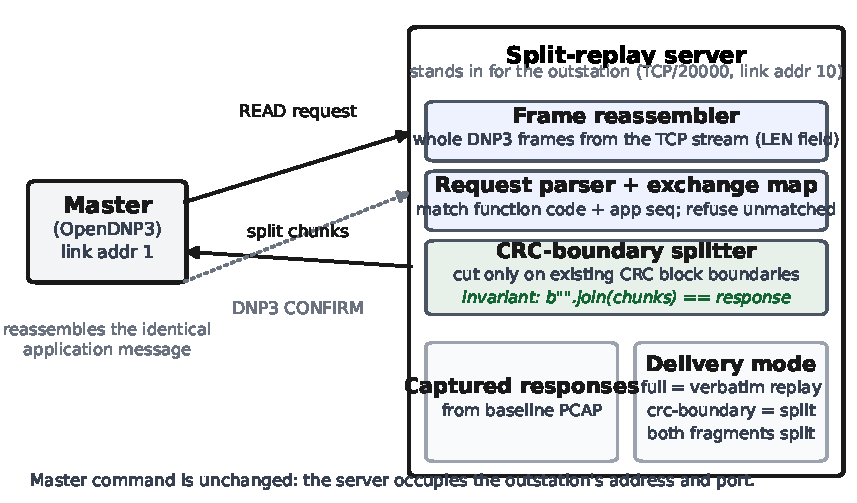
\includegraphics[width=0.86\textwidth]{figures/fig1_architecture.pdf}
\caption{The request-aware split-replay server stands in for the outstation. It
reassembles whole DNP3 frames from the TCP stream, matches each request to its
captured response, splits data responses only on existing CRC block boundaries,
and preserves the CONFIRM handshake. The master command is unchanged.}
\label{fig:arch}
\end{figure*}

\noindent\textbf{The primitive.} CRC-boundary splitting slices a captured DNP3
response into TCP chunks strictly along the seams between its CRC-protected
blocks. To split one response, we walk it into its run of blocks, i.e., the
10-byte link header block and then the 16-byte data blocks, each closed off by
its CRC, and we pack a chosen number of whole blocks into each TCP chunk. Since a
chunk always opens and closes on a block boundary, it ends on a CRC that is
already valid, and the chunks reassemble into the original response. The server
checks the byte-preservation invariant \code{b"".join(chunks) == response} before
it sends anything, and it refuses to send when the check fails. The upshot is
that no DNP3 byte moves, no CRC is recomputed, and no length field is touched, so
the master's link-layer and transport-layer reassembly runs exactly as it does
for the untouched response.

\noindent\textbf{How aggressively to split.} The number of whole blocks per chunk
is the one knob that sets how finely the response is broken up. Set it to one and
every CRC block becomes its own TCP segment, which is as aggressive as a
byte-preserving split can get; raise it and more blocks ride in each write,
giving a coarser split. Going finer than one block per chunk is off the table,
because it would mean cutting inside a CRC block, which snaps a boundary and steps
outside the byte-preserving primitive. The server can also hold each chunk back
by a set interval, so the timing side of the fingerprint moves independently of
the size side.

\noindent\textbf{Replaying with the request in view.} The split-replay server
occupies the outstation's own address and port, which is why the master command
never changes. To answer correctly without carrying a full DNP3 stack, the server
rebuilds whole DNP3 frames from the TCP stream off the link-header length field,
reads out each request's function code and application sequence, and replies with
only the captured response tied to that request. A captured session carries
startup and handshake exchanges alongside the data read, so matching every
request to its own captured response keeps the master on the trajectory it
followed in the capture. The server will not fire a captured response at a request
it cannot match, which shuts down the blind byte-dumping that an earlier,
positional replay design fell into. Only the data responses are split on CRC
boundaries; the short handshake replies go out whole.

\noindent\textbf{Multi-fragment responses and the CONFIRM.} A large read comes
back in more than one application fragment. The outstation sends the first
fragment, the master answers with a DNP3 CONFIRM, and only then does the
outstation send the continuation. The server keeps that handshake: it sends the
split first fragment, waits on the master's CONFIRM bytes, and then sends the
continuation, split on its own CRC boundaries. As a result the continuation is
obfuscated just as much as the first fragment, rather than slipping out as one
write.

\section{Implementation}

The harness is written in Python around an OpenDNP3~\cite{ref:opendnp3} outstation
and master, reached through the ChargePoint pydnp3 binding. The outstation runner
(\code{run\_outstation.py}) brings up a real OpenDNP3 outstation with a
configurable database, turns unsolicited responses off, and refuses controls by
default, so a baseline capture holds nothing but the reads we issued. The master
runner (\code{run\_master.py}) sends one controlled Class~0 read and writes the
measurements it gets back to a per-phase CSV, along with a measurement receipt
meant for a human to read. Every lab setting, i.e., host addresses, TCP port, and
DNP3 link addresses, comes out of a single configuration module, so no address is
ever typed on the command line.

The split-replay server (\code{split\_server.py}) carries no DNP3 stack at all.
Inside it are a frame reassembler, a request parser, the CRC-boundary splitter,
and a captured-exchange map, and it leans on nothing but itself and the
configuration module. Two delivery modes are on offer: \code{full} replays each
captured response verbatim, while \code{crc-boundary} splits every data response
along its CRC boundaries. The byte-preservation check runs over each response
before it leaves. We hold the harness inside the byte-preserving phase on purpose:
it recomputes no CRC, edits no DNP3 field, adds no padding, and runs no live
proxy, which keeps byte preservation the invariant we can always point to.

\section{Evaluation}

Here we put CRC-boundary splitting through the testbed. Three questions drive the
evaluation. First, how does an OpenDNP3 outstation segment its own responses,
i.e., what is the fingerprint we are trying to blur? Second, does the master
still accept and correctly reassemble a response after it has been split on CRC
boundaries? Third, how far can the size and segmentation of a response be pushed
while byte-level acceptance still holds?

\noindent\textbf{Testbed.} Two hosts sit on a 1~Gb/s management network, switched
directly to each other. The master runs on one; the outstation, or the
split-replay server standing in for it, runs on the other on TCP port~20000. DNP3
link addresses are 1 for the master and 10 for the outstation. We capture on the
master's interface behind a port filter and read the captures with scapy and a
DNP3 CRC helper. Both ends run OpenDNP3 through pydnp3 on Python~3.12. Unless we
say otherwise, every result below comes off the two-host rig rather than loopback.

\subsection{The native segmentation fingerprint}

To pin down the fingerprint, we fire a single large Class~0 read at an outstation
set up with 200~analog, 50~binary, and 50~counter points, and we read the
response out of the capture. Table~\ref{tab:baseline} lays out what came back. The
outstation returns a 12{,}204-byte response carried as 9~application fragments,
49~link frames, and 20~TCP segments. Of those 49~link frames, 46 sit at the
292-byte DNP3 maximum and the rest are short per-fragment tails. The response
reaches 49~link frames for a simple reason: 292~bytes is the DNP3 link-frame
ceiling, so a long application fragment has no choice but to travel as a run of
full frames plus a short tail.

\begin{table}[t]
\centering
\caption{Native segmentation of a large Class~0 read (200 analog + 50 binary +
50 counter).}
\label{tab:baseline}
\begin{tabular}{@{}p{0.62\columnwidth}r@{}}
\toprule
Layer & Result \\
\midrule
Total response bytes (outstation to master) & 12{,}204 \\
DNP3 application fragments (transport FIR/FIN) & 9 \\
DNP3 link frames (\code{0x0564}) & 49 \\
Link frame sizes & $46 \times 292$\,B + tails \\
TCP segments (response) & 20 \\
\bottomrule
\end{tabular}
\end{table}

The DNP3 layer and the TCP layer cut the stream on their own schedules. The kernel
packs the link frames into TCP segments of up to 1448~bytes, i.e., the
connection's maximum segment size, so one 292-byte link frame can spill across a
TCP segment boundary and one TCP segment can hold several partial link frames. The
two boundaries, in other words, do not line up, and the pattern on the wire
carries both the DNP3 frame structure and the TCP packing at once.

To check that the fingerprint really tracks the database, we sweep the read range
over a 200-analog database and measure the response at each range.
Table~\ref{tab:range} lays out the result. The response grows in a straight line,
close to 5.7~bytes for every analog point, and the frame and segment counts climb
once the response clears the 292-byte frame ceiling and the maximum segment size.
So a passive observer can read how many points a device carries straight off the
size and segmentation of its response, and that is the fingerprint CRC-boundary
splitting sets out to blur. An observer might well fold the response timing in
with the size estimate to sharpen the fingerprint further.

\begin{table}[t]
\centering
\caption{Response size versus read range on a 200-analog database.}
\label{tab:range}
\begin{tabular}{@{}lrrrr@{}}
\toprule
Read range & Analog pts & Bytes & Link frames & TCP segs \\
\midrule
0..9   & 10  & 129   & 4 & 4 \\
0..49  & 50  & 332   & 3 & 3 \\
0..99  & 100 & 625   & 4 & 3 \\
0..199 & 200 & 1{,}211 & 6 & 3 \\
\bottomrule
\end{tabular}
\end{table}

We also look at how the outstation behaves at the TCP level on that same large
read. It piggybacks the application response on the TCP acknowledgment for 9 of
9~requests, the mean request-to-acknowledgment delay sits at 0.24~ms and the mean
request-to-response delay at 1.01~ms, and the steady-state data segments carry a
\code{NOP-NOP-Timestamp} TCP option signature. That is the host's TCP/IP stack
fingerprint, a separate thing from the DNP3 application fingerprint, and it would
come out differently for a field device on a different stack.

\subsection{Does the master accept a split response, and are the measurements
right}

To find out whether the master accepts a split response, we run the whole pipeline
on the rig. First we capture a baseline read against the real outstation and pull
the captured responses out; then we swap the outstation for the split-replay
server and run the read again, once with verbatim replay and once with
CRC-boundary splitting. We line the delivered measurements up across the three
runs.

The master takes the split response and rebuilds the identical application
message. A captured 2{,}407-byte read response, which OpenDNP3 natively carries as
9~link frames, goes out as 141~chunks of at most 18~bytes under one-block-per-chunk
splitting, and the master still delivers all 800~measurements from the replayed
response set and answers with a DNP3 CONFIRM. The measurement sets agree at three
levels. The split bytes concatenate back to the original response, which is the
byte level. The master flags no DNP3 parser or CRC error and sends the CONFIRM,
which is the protocol level. And the delivered measurements match the baseline,
which is the measurement level. We also ran a clean-pipeline check on a Class~0
read that returned 2{,}400 unique measurement tuples across a 6-fragment response;
the baseline, the verbatim replay, and the CRC-boundary split all produced
byte-identical measurement sets, with every data fragment split and the handshake
replies left whole. The measurements survive because CRC-boundary splitting moves
only where the TCP write boundaries land, which the master's reassembly does not
care about, and leaves every DNP3 byte and CRC exactly where it was.

\subsection{How far the fingerprint can be pushed}

To see how far the fingerprint can be pushed, we replay that same captured
2{,}407-byte response split at one, two, four, and eight blocks per chunk, with
everything else held fixed. Table~\ref{tab:sweep} lays out the result, and
Fig.~\ref{fig:split} sets the distortion against the native response.

\begin{figure*}[t]
\centering
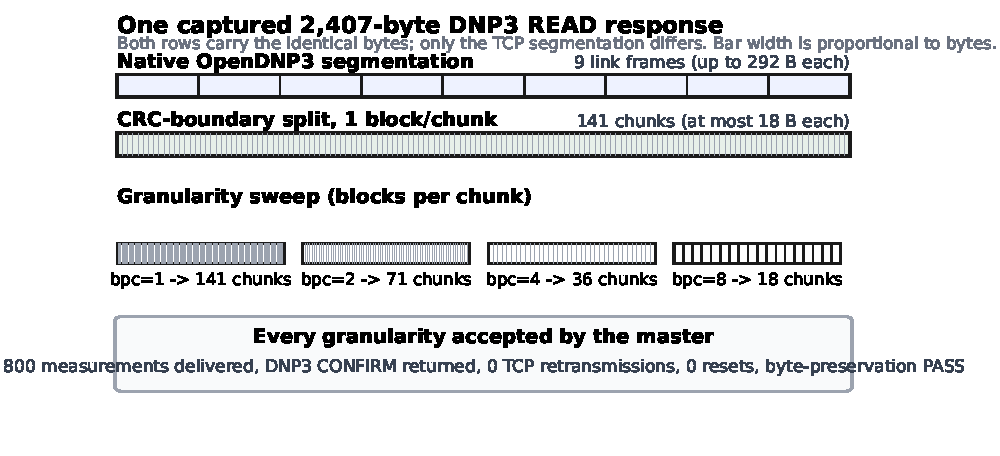
\includegraphics[width=0.86\textwidth]{figures/fig2_baseline_vs_split.pdf}
\caption{The same 2{,}407-byte response carries the identical bytes in both rows;
only the TCP segmentation differs. OpenDNP3 natively presents it as 9~link
frames, while one-block-per-chunk CRC-boundary splitting presents it as
141~chunks of at most 18~bytes. Across the granularity sweep the master accepted
every level, delivering all 800~measurements with a CONFIRM on a clean
connection.}
\label{fig:split}
\end{figure*}

\begin{table}[t]
\centering
\caption{Split-aggressiveness sweep on a captured 2{,}407-byte READ response
(9 native link frames).}
\label{tab:sweep}
\begin{tabular}{@{}rrrrrr@{}}
\toprule
Blocks/chunk & Chunks & Meas. & CONFIRM & Retx & Resets \\
\midrule
1 & 141 & 800 & yes & 0 & 0 \\
2 & 71  & 800 & yes & 0 & 0 \\
4 & 36  & 800 & yes & 0 & 0 \\
8 & 18  & 800 & yes & 0 & 0 \\
\bottomrule
\end{tabular}
\end{table}

The master accepts every granularity and hands back all 800~measurements. It
returns a CONFIRM over a connection with no retransmission and no reset, while the
READ response goes out as 141, 71, 36, and 18~chunks in turn. The chunk counts
land on the ceiling of 141 over the blocks-per-chunk value, exactly. So the
byte-preserving obfuscation envelope runs the full block-grouping range, and the
sharpest distortion in size and segmentation lands at one block per chunk, where a
single 2{,}407-byte response the outstation would show as 9~frames instead shows
as 141~tiny segments. Push fragmentation past that point, or move per-frame sizes
around at will, and you are back to rebuilding frames and recomputing CRCs, which
is outside the byte-preserving primitive.

\section{Discussion}

\noindent\textbf{From harness to a deployed defense.} The harness settles the
primitive in software, where the split-replay server stands in for the outstation
and replays captured responses. It is not yet the in-network implementation. A
deployed defense would run CRC-boundary splitting over live responses in the data
plane, say on a programmable switch, rather than over captured ones. That
in-network, live build, and the throughput and latency numbers that come with it,
we leave for later.

\noindent\textbf{What it hides, and what it does not.} CRC-boundary splitting
bends the size and segmentation of a response, and through the chunk delay its
timing, while the DNP3 bytes stay put. What it does not bend is the total byte
count the application response carries, so an observer that tallies total payload
bytes across a full exchange can still get at the read size. Making the total size
itself less telling calls for padding or frame rebuilding, both of which recompute
CRCs, and that is a separate line from the byte-preserving primitive we study
here. A padding-based extension, and how it would sit with the master's
reassembly, we leave for later.

\noindent\textbf{How far the evaluation reaches.} Our fingerprinting numbers
describe one outstation on one testbed, so they show what the primitive changes on
the wire, not a measured drop in an adversary's ability to classify devices apart.
A fingerprinting study spread across device types and stacks would let us state
the obfuscation effect as a fall in classification accuracy. That study, too, we
leave for later.

\section{Related Work}

\noindent\textbf{Obfuscating ICS traffic against reconnaissance.} Earlier work
obfuscates control-network communication to throw off an adversary's
reconnaissance of power grids. In~\cite{ref:raincoat}, the authors randomize data
acquisitions and craft decoy measurements to steer attackers into ineffective
strategies, and in~\cite{ref:defrec}, the authors virtualize physical devices to
disrupt reconnaissance of the cyber-physical infrastructure. Both blur the content
and the connectivity an adversary learns. This work chases a different target: it
blurs the wire-visible size and segmentation of a DNP3 response without touching a
single application byte, so it sits alongside content-level obfuscation rather
than standing in for it.

\noindent\textbf{Fingerprinting encrypted traffic, and shaping it back.} A wide
line of work fingerprints encrypted traffic off packet sizes and timing, then
fights back with padding and by reshaping the packet-size
distribution~\cite{ref:fp}. The size and segmentation of DNP3 responses hand over
a comparable side channel, only in an unencrypted industrial setting. Set against
general traffic-shaping defenses, CRC-boundary splitting is boxed in by the DNP3
CRC structure: it can re-segment as it likes on block boundaries but cannot move
bytes or sizes without recomputing CRCs, so it trades some reshaping room for
exact byte preservation and a master that accepts the result without noticing.

\noindent\textbf{Watching DNP3 for attacks.} Other work bolts intrusion detection
and specification-based monitoring onto DNP3 traffic~\cite{ref:bro}, and studies
the safety fallout of malicious DNP3 commands~\cite{ref:cps}. Those efforts detect
or analyze malicious activity in the traffic. This work is not a detection
technique at all: it reworks the outstation's observable traffic to resist passive
fingerprinting, ahead of any malicious activity.

\section{Conclusion}

A passive observer can fingerprint a DNP3 outstation off the size, segmentation,
and timing of its responses, cues that hold steady because the outstation segments
deterministically and any byte change trips the protocol's CRCs. This paper put
forward CRC-boundary splitting, a byte-preserving primitive that re-segments a
captured response only along its existing CRC block boundaries, and built it into
a request-aware split-replay server. On a two-host testbed the master accepted
every splitting granularity and returned measurements identical to the baseline,
while a response OpenDNP3 shows natively as 9~frames went out as up to 141~tiny
segments over a connection with no retransmission and no reset. We take that as
reason to believe CRC-boundary splitting can carry an in-network obfuscation layer
as its transparent primitive, and building that layer into the data plane is where
we go next.

% -------------------------------------------------------------------------
% NOTE: the references below are PLACEHOLDERS. Replace each with a complete,
% verified citation before submission. The text names the intended source.
% -------------------------------------------------------------------------
\begin{thebibliography}{1}

\bibitem{ref:dnp3}
IEEE Standard for Electric Power Systems Communications --- Distributed Network
Protocol (DNP3), IEEE Std 1815. [complete citation]

\bibitem{ref:ukraine}
Analysis of the December 2015 Ukraine power grid cyberattack (e.g., E-ISAC/SANS
report). [complete citation]

\bibitem{ref:raincoat}
H.~Lin, Z.~Kalbarczyk, and R.~K. Iyer, ``RAINCOAT: Randomization of network
communication in power grid cyber infrastructure to mislead attackers,'' IEEE
Trans. Smart Grid. [complete citation]

\bibitem{ref:defrec}
H.~Lin \emph{et al.}, ``DefRec: Establishing physical function virtualization to
disrupt reconnaissance of power grids' cyber-physical infrastructures,'' NDSS.
[complete citation]

\bibitem{ref:fp}
Representative website/traffic fingerprinting attack and padding-based defense.
[complete citation]

\bibitem{ref:bro}
H.~Lin \emph{et al.}, ``Adapting Bro into SCADA: Building a specification-based
intrusion detection system for the DNP3 protocol.'' [complete citation]

\bibitem{ref:cps}
H.~Lin \emph{et al.}, ``Safety-critical cyber-physical attacks: Analysis,
detection, and mitigation.'' [complete citation]

\bibitem{ref:opendnp3}
OpenDNP3, an open-source implementation of the DNP3 protocol stack. [complete
citation]

\end{thebibliography}

\end{document}
